% Generated from iab2026-draft.md (the source of truth). Do not edit in place —
% change the draft, then regenerate. Sections awaiting the re-run are marked
% GAP and left deliberately empty rather than filled with retired numbers.
\documentclass[10pt]{article}
\usepackage[letterpaper,margin=1in,top=0.85in]{geometry}
\usepackage{fontspec}
\usepackage{xeCJK}
\setmainfont{Times New Roman}
\setCJKmainfont{Songti SC}
\usepackage{amsmath,amssymb}
\usepackage{graphicx}
\usepackage{booktabs}
\usepackage{caption}
\usepackage[hidelinks]{hyperref}
\usepackage{titlesec}
\usepackage{xcolor}
\titlespacing*{\section}{0pt}{6pt}{2pt}
\titlespacing*{\subsection}{0pt}{5pt}{2pt}
\titleformat*{\section}{\large\bfseries}
\titleformat*{\subsection}{\normalsize\bfseries}
\captionsetup{font=small,labelfont=bf,skip=4pt}
\setlength{\parskip}{1pt}
\usepackage{enumitem}
\setlist{nosep,leftmargin=1.3em}

\title{\bfseries Thinking Sideways, Observed:\\ Interpreting the Lateral-Thinking Search Behavior of LLM Agents}
\author{Xiaoxuan Lei \and (co-authors TBD)\\
\small Draft v0.13 --- IAB: Interpreting Agent Behavior, Workshop @ NeurIPS 2026}
\date{}

\begin{document}
\maketitle
\vspace{-1.8em}

\begin{abstract}
\small\noindent An endpoint score records where an agent's search ended, not
how it moved, and one flat score can hide opposite failures. We instrument
Turtle Soup, a lateral-thinking game of yes/no questions, with two
process-level probes, a forced and scored checkpoint story every round and an
association trajectory embedded from each round's question, and run three Qwen
tiers on 22 human-played puzzles. The endpoint story is flat: gains occur only
in the first ten of thirty rounds and only at the larger tiers, and the round
budget is not the constraint (the smallest tier's apparent decline under
longer caps is a token-exhaustion harness artifact that our own audit rule
catches). Beneath that one flat curve sit two opposite patterns. The small
model \emph{circles} one hypothesis, its late-game stride under half the
mid-size tier's (0.030 vs 0.082, cluster-robust and unchanged when its
malformed rounds are excluded); the largest tier \emph{abandons}, committing
only 1 of its 6 solution-grade games while four of them end below half their
peak. The geometry describes these failures but does not predict scores:
within puzzles every stride and drift coefficient is bounded near zero
(smallest LRT $p = 0.097$, both anchors). Finally, endpoint scores cannot even
attribute failure: in a pilot, repairing a 30\%-accurate Oracle to 100\% left
the smallest Questioner's score unchanged, so attribution in either direction
requires auditing and intervening on the environment, a doctrine this paper
applies to its own results twice. We release the harness, both instruments,
the provenance-enforced puzzle set, and every per-game log.
\end{abstract}

\section{Introduction}
Here is a Turtle Soup puzzle. \emph{A man's body lies in the desert, clutching half
a matchstick; luggage and clothing are scattered around him.} That is all the
solver sees. The hidden story: a hot-air balloon was losing altitude; the
passengers threw out their luggage, still could not stay up, and drew lots with
matchsticks; the man who drew the short one was thrown out. The solver recovers
this story by asking yes/no questions, one per round.

Outcome metrics can say whether an agent got there; on our set that story is
flat, and the round budget is not the constraint (\S\ref{sec:results}). What
they cannot say is how the agent searched: one zero-scorer never leaves its
first hypothesis, another finds the answer and lets it go. Instruments that
read the process, and an environment audited enough to trust them, are this
paper's contribution. Turtle Soup suits the job: the behavior \emph{is} text
(no activation access needed), puzzles are deliberately under-determined so
each associative jump's direction is diagnostic, and games are short and
cheap at scale.

\textbf{Three questions.} We embed each round's question in a semantic space
and ask: \textbf{Q1}, does an agent that fails circle a hypothesis basin, its
stride (per-round semantic step size) shrinking toward zero, of which lexical
novelty catches only the verbatim extreme? \textbf{Q2}, does it instead drift,
striding normally while moving away from the anchor? \textbf{Q3}, do such
trajectory features predict solve quality? The answers are yes (we name the
pattern \emph{circling}), no, and no; and the checkpoint record reveals a
second pattern the geometry did not hypothesize, \emph{abandoning}
(\S\ref{sec:results}).

\textbf{Contributions.} (1)~Two process-level instruments for interactive
agents: a forced-checkpoint and commitment protocol that scores a complete
answer every round, and an association-trajectory geometry, with an honest
account of what each does and does not show. (2)~An environment-first audit
doctrine, demonstrated twice: an Oracle pilot showing endpoint scores cannot
attribute failure to agent or environment, and a token-exhaustion dissection
that demotes one of our own headline declines to a harness artifact.
(3)~Two operationalized failure patterns, \emph{circling} and
\emph{abandoning}, with per-game criteria and counts, under one flat endpoint
score. (4)~A released harness, a 22-puzzle set restricted to puzzles humans
have played and solved, per-game logs, and a two-part score whose halves
correlate only weakly per game ($\rho \leq 0.35$); the set's
under-determination difficulty measure is rounds-independent, though not yet
predictive of outcomes (\S\ref{sec:results}).

\section{Related Work}\label{sec:rw}
Existing turtle-soup benchmarks, TurtleBench~\cite{turtlebench},
SPLAT~\cite{splat} (whose interactive player--judge protocol we adopt), and
TurtleSoup-Bench~\cite{tsbench}, score verification accuracy, solve efficiency,
or faithfulness to the intended story. TurtleSoup-Bench probes what agents ask
next but grades it against the intended story; none of the three measures the
search's geometry, which is our delta. Circling and abandoning echo folk-known
multi-turn failure modes (repetitive questioning; failing to commit or retain
a correct answer); our contribution is to measure them, not to claim their
novelty. MUTATE~\cite{mutate} shows frontier agents find far fewer mechanism-distinct
paths than humans; its diverge-then-narrow agent is a natural test
intervention for our metrics. The instrument itself adapts
forward flow~\cite{forwardflow} and the Divergent Association
Task~\cite{dat} from human psychometrics. The Small World of Words
norms~\cite{swow} provide the human anchor that ours is not yet
(\S\ref{sec:framework}). Judge-bias
catalogues~\cite{calm,posbias} shape the scoring: the model judge is confined
to the one subscore that objective matching cannot reach.

\section{Framework}\label{sec:framework}
\subsection{Task and harness}
A \textbf{Questioner} sees only the 汤面 (the ``surface'', the puzzle's visible
scenario) and asks one yes/no question per round. An \textbf{Oracle} holds the
汤底 (the hidden story) and answers 是/不是/与此无关 (yes, no, or
irrelevant). The Questioner may
commit a final story at any round, or is forced to at the budget. The
open-source harness has pluggable model providers and logs every round, with
per-game seeds.

\subsection{Checkpoint and commitment instrumentation}\label{sec:checkpoint}
Our first instrument does not wait for the end. Every round, after the Oracle
answers, the Questioner must write its best complete story, and \emph{that}
checkpoint is scored; each point on an accuracy curve is therefore a full
answer written with the evidence available at that round. Alongside it we
record \emph{commitment}: whether and when the agent ever volunteers a final
story of its own accord. Together these turn an endpoint benchmark into a
scored process.

\subsection{Puzzles}
A puzzle nobody has solved carries no evidence that its clues suffice, that its
solution is unique, or that the intended leap is reachable; an agent scoring zero
on it teaches us nothing. Our set therefore takes only puzzles with a public
record of human play: 22 items from a Chinese Turtle Soup community site, each
keeping its source URL. Surfaces run 9--108 characters (median 34), solutions
13--200 (median 102), with 97 annotated key clues. Provenance is enforced in
code, with a verified family, a quarantined generated family, and tests that
fail if the two mix.

Each puzzle carries an \textbf{under-determination} score: how far the surface
alone leaves a solver from the solution, measured by taking the closest of
twelve cold guesses written from the surface with no Oracle feedback. It
ranges 0.173--0.577 (median 0.347) over the set and is \emph{not} explained by
surface length within this small set ($r=-0.22$, n.s., $n=22$). It enters the mixed-effects
analysis in \S\ref{sec:results} as a puzzle-level covariate.

\subsection{Outcome scoring: composite, not surface}
Judged outcome is \textbf{clue recall (70)} plus \textbf{causal-logic identity
(30)}; Appendix~\ref{app:metrics} gives the detail. String matching alone cannot
tell a wrong answer from a right one worded differently: we watched a frontier
model reconstruct a hidden causal chain completely and score $0.00$. Conversely,
the clue half blocks ``far $=$ creative'' gaming, because distance without
validity scores zero.

\subsection{Association-trajectory instrumentation}\label{sec:traj}
The second instrument reads the questions themselves. Each round, we extract
the question's keywords (jieba), embed them (bge-small-zh-v1.5), and average
them to a unit round vector $q_t$; distances are cosine, and anchors embed the
puzzle's surface, solution, and clue terms (specification in
Appendix~\ref{app:metrics}). Two signals follow: the \textbf{stride}
$s_t = d(q_t,q_{t-1})$ and the \textbf{anchor distance}
$h_t = d(q_t,\mathcal{A})$, with Q1's signature $\bar{s}\to 0$ and Q2's a
rising $h_t$; the lexical \texttt{question\_novelty} metric is the ablation
baseline that Q1 predicts will miss synonym drift. One caveat up front: the
anchor is a stated proxy, not a human association manifold; its consequences
are quantified with the results (\S\ref{sec:results}), and a SWOW-based
version~\cite{swow} is the correct future form.

\begin{figure}[t]
\centering
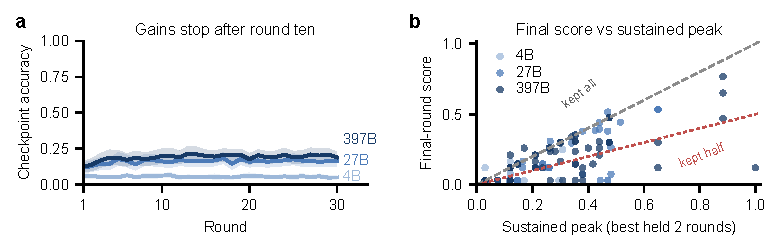
\includegraphics[width=0.58\linewidth]{figures/fig1_flatness.pdf}
\caption{\textbf{(a)}~Mean checkpoint accuracy by round on the full 0--1
range (bands, 95\% cluster-bootstrap CIs over the 22 puzzles); dashed rule at
round 10; inset magnifies the early rise. \textbf{(b)}~Final score against
sustained peak, one point per E1 game; filled markers are games whose final
story was volunteered, open markers were never committed, and the dashed
vertical rule marks solution-grade peaks ($\geq 0.5$; points may sit above
the diagonal since the peak needs two consecutive rounds).}
\label{fig:e1}
\end{figure}

\section{Experiment Designs}
\textbf{Designs.} E1 (round curve) plays to 30 rounds under the checkpoint
instrument (\S\ref{sec:checkpoint}). E2 (round budget) imposes hard caps
$\{5,10,15,20,25,30\}$ with a forced final answer only, so it doubles as a
no-checkpoint control. E3 (association trajectory) computes $\{s_t\}$ and
$\{h_t\}$ for every E1 game and answers Q1--Q3; the keyword extractor is
fixed across models, so none is scored through its own vocabulary.

\textbf{Prerequisite: the Oracle audit.} The Oracle is the sole information
channel: a weak one collapses answers to ``irrelevant'', after which no
Questioner can succeed and every score measures the environment. In a pilot, a
4B Oracle (thinking disabled) answered 30\% of probes correctly; substituting
a 100\%-accurate Oracle left the 4B Questioner's score unchanged. The lesson:
an endpoint score cannot say which side failed (here the environment was not
the bottleneck); only audit plus intervention licenses attribution either way.
Candidates are therefore probed on 25 held-out (question, answer) pairs over
three puzzles before any agent claim (protocol and per-candidate numbers in
Appendix~\ref{app:metrics}), and \textbf{must come from a different model
family than the Questioners}, or a Questioner's resemblance to the Oracle
cannot be separated from its tier.

\section{Results}\label{sec:results}
All numbers come from one grid on the verified set: 22 puzzles $\times$
\{Qwen3.5-4B, Qwen3.6-27B, Qwen3.5-397B-A17B; hereafter 4B, 27B, 397B\}
$\times$ 3 seeds, with a DeepSeek-V3.1 Oracle and logic judge (cross-family
with the Questioners; audit and settings in Appendix~\ref{app:metrics}). The
three models differ in generation and architecture (the 397B is a
mixture-of-experts with 17B active parameters), so we speak of model tiers,
not scale; harness failures were zero, and token exhaustion is a game outcome
reported below. Accuracy denotes the composite score rescaled to $[0,1]$. E1
comprises 198 thirty-round games with a scored checkpoint every round; E2,
1{,}188 games across caps $\{5,10,15,20,25,30\}$. Circling will emerge from
the geometry (\S\ref{sec:patterns}); abandoning from the checkpoint record
(\S\ref{sec:e1}, \S\ref{sec:patterns}).

\subsection{More interaction stops helping after ten rounds (E1)}\label{sec:e1}
Checkpoint accuracy rises only in the first ${\sim}10$ rounds, and only for
the larger tiers: 397B climbs from $0.124$ (round 1) to $0.200$ (round 10),
then stays between $0.18$ and $0.21$; 27B rises $0.117 \to 0.162$ and plateaus
near $0.16$; 4B is flat at $0.05$--$0.06$ throughout (Figure~\ref{fig:e1}a).
The round 10 to 30 change is $-0.009$ / $+0.003$ / $-0.013$ across tiers
(puzzle-clustered 95\% CIs spanning or hugging zero). E1 imposes no game
token budget (the 50k budget governs E2 play) and no E1 game ended early, so
the curves carry no survivorship.

\textbf{Commitment: abandoning's first evidence.} 27B volunteers a final story
in 11/66 games (mean round 11.1), 397B in 9/66 (14.2), and 4B in 2/66 (23.5);
the smallest neither improves nor concludes, and the largest, as
\S\ref{sec:patterns} quantifies, finds and does not commit.

\textbf{Peaks, finals, and an honest null.} Model tier raises what is found
mid-game: the \emph{sustained} peak (best score held over two consecutive
checkpoints, robust to single-round rewording swings) averages 0.084 / 0.240 /
0.296 across tiers, while finals sit lower (Figure~\ref{fig:e1}b). Retention
(final over sustained peak; estimator and inclusion rules in
Appendix~\ref{app:metrics}) is 0.69--0.76 at every tier, yet under a
within-game permutation null (knowledge constant, only scoring jitter) it is
expected at 0.79--0.84, and the observed values are not significantly below
($p \geq 0.09$). The quantitative case for ``finding and losing'' is
therefore inconclusive; abandonment's evidence is the commitment record above
and \S\ref{sec:patterns}'s cross-tabulation.


\subsection{Budget pressure and a harness artifact (E2)}\label{sec:e2}
End accuracy is insensitive to the round cap for the larger tiers (397B
$0.19$--$0.21$ and 27B $0.14$--$0.18$ across all six caps). The smallest
model's raw curve declines monotonically ($0.050$ at cap~5 to $0.004$ at
cap~30), but this is an environment effect, not a behavioral one: games ending
by token-budget exhaustion rise from 0/66 at cap~5 to 63/66 at cap~30 (175 of
396 overall, versus 2/396 for 27B and 0/396 for 397B), and conditioned on
non-exhausted games 4B's end accuracy does not decline (0.05--0.09 across
caps). By our own audit principle, the raw decline measures the harness. This
resolves an internal check: 4B's E1 round-30 mean (0.05) and E2 cap-30 final
(0.004) differ exactly by exhaustion; on non-exhausted games the protocols
agree, as at the larger tiers.

\textbf{The two score halves dissociate} (a scoring-instrument check on E2's
games). Every model earns proportionally far more of the judged causal-logic
half than the clue-recall half: 397B averages
12.6/30 logic against 7.2/70 clues, 27B 10.1 against 6.8, and 4B 2.9 against
0.2, and the halves correlate only weakly per game (Spearman $\rho = 0.30$ /
$0.35$ / $0.06$ for 397B / 27B / 4B). Models reach the right causal shape
well before, and often without, landing the annotated clue content; the logic
half is not redundant with string-level recall.

\begin{figure}[t]
\centering
\begin{minipage}[t]{0.545\linewidth}
\centering
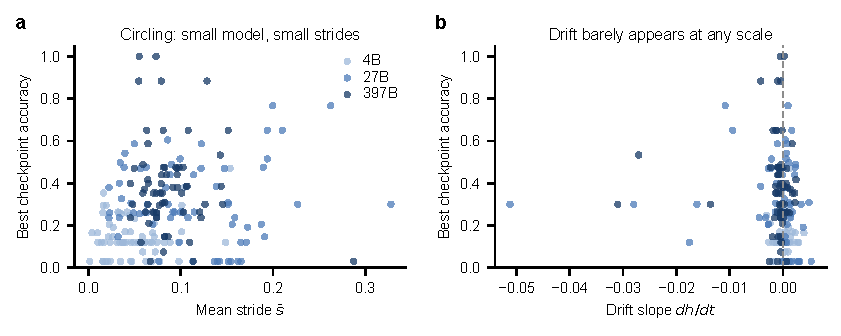
\includegraphics[width=\linewidth]{figures/fig2_geometry.pdf}
\captionof{figure}{Per-trace geometry ($n = 198$). \textbf{(a)}~Per-game mean
stride by tier (dots; bars, tier mean $\pm$ 95\% CI): 4B sits below the
larger tiers. \textbf{(b)}~Drift slope against best accuracy, clustered near
zero at every tier: Q2's absent signature.}
\label{fig:e3}
\end{minipage}\hfill
\begin{minipage}[t]{0.425\linewidth}
\centering
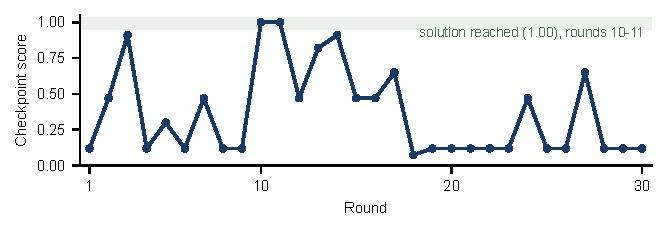
\includegraphics[width=\linewidth]{figures/fig3_worked.pdf}
\captionof{figure}{One abandoning game (\texttt{refsoup\_021}, 397B, seed 2):
the round 10--11 checkpoint stories are the solution (band), never
volunteered, abandoned by round 19. Bilingual rows in
Appendix~\ref{app:metrics}.}
\label{fig:worked}
\end{minipage}
\end{figure}

\subsection{Two patterns: circling and abandoning (E3)}\label{sec:patterns}
With the environment artifact removed, the differences are behavioral.
\textbf{Circling} (Q1, confirmed): 4B's mean stride is $0.049$
$[0.040, 0.060]$ against $0.114$ (27B) and $0.088$ (397B); its late-game
stride (second half) is $0.030$ $[0.021, 0.039]$ vs 27B's $0.082$
$[0.065, 0.098]$ (puzzle-clustered 95\% CIs; Figure~\ref{fig:e3}a). Not a
malformed-question artifact: 17\% of 4B's questions are truncated or
non-interrogative (${\sim}1\%$ elsewhere), yet excluding them barely moves
either statistic ($0.049 \to 0.056$; $0.030 \to 0.033$). Stride separates 4B
from the larger tiers, whose own order is non-monotonic.

\textbf{Abandoning} (unhypothesized; from the checkpoint record): call a
sustained peak $\geq 0.5$ (half the scale) \emph{solution-grade}. 4B reaches
none; 397B reaches six, commits one, and ends four below half peak (ratios
0.12--0.87); 27B reaches four, commits three, keeping ${\sim}0.83$.
Abandoning concentrates in the largest tier; Figure~\ref{fig:worked} shows
one game whole. Under per-game criteria (circling: late stride $<0.04$, no
commit, no peak $\geq 0.3$; abandoning: peak $\geq 0.3$ ending below half),
the tiers swap dominant failures (4B, 39 vs 1 of 66; 397B, 6 vs 12), no game
meeting both.

\textbf{Drifting} (Q2, rejected): slopes cluster near zero at every tier
(Figure~\ref{fig:e3}b). In language space, lexical novelty catches only 4B's
verbatim re-asks, scores fresh-worded re-asks of one hypothesis as new, and
cannot see abandoning at all.

\textbf{Predictivity} (Q3, not supported): pooled across tiers, stride
correlates with best score ($\rho = 0.23$, $n = 198$), a between-tier effect;
within tiers none is detected ($|\rho| \leq 0.16$). A mixed-effects model
(specification and coefficients in Appendix~\ref{app:metrics}) detects no
stride or drift effect, every coefficient within $\pm 0.035$ per SD, smallest
LRT $p = 0.097$; the under-determination covariate is likewise n.s.
($p = 0.22$, ${\sim}8\%$ of puzzle variance), so the puzzle effect is not
merely measured difficulty. Effects are bounded small, not excluded: the
geometry is an interpretive instrument, saying \emph{how} an agent fails, not
a score predictor. Because the anchor overlaps the clue set, everything is
computed twice: slopes from the two anchors agree in rank ($\rho = 0.80$) yet
flip sign on 38/198 traces, and the conclusion is unchanged though weaker
surface-only ($\beta = -0.020$ $[-0.044, 0.003]$, $p = 0.097$); the anchor
changes traces, not the finding.


\section{Limitations and Conclusion}
\textbf{Limitations.} Truncated chain-of-thought under a tight token budget
masquerades as an agent that cannot form a question
(\S\ref{sec:e2}, \S\ref{sec:patterns}); decoding is part of the environment,
and the Oracle's ${\sim}95\%$ audited accuracy implies roughly one wrong
answer per 30-round game, an unmeasured environment term. The anchor is not yet human-derived (\S\ref{sec:traj}), so
Q2's framing is descriptive until SWOW norms or human traces exist. Keyword
extraction and encoders are themselves
models; feedback incorporation, the most direct separator of the two
patterns, is unmeasured. One DeepSeek model serves as both Oracle and judge
(cross-family judge check pending), and the tiers
confound generation and architecture, so tier effects are model comparisons,
not scaling laws. The source site is public and memorisation probes are pending; nothing rests
on the n.s.\ under-determination covariate. Puzzles involve death and dark themes; content-flagged.

\textbf{Conclusion.} Under these flat curves sit two opposite failures
needing opposite interventions; telling them apart took both instruments and
an audited environment. Geometry exposes circling; the checkpoint record,
abandoning; the score, neither.

\begin{thebibliography}{9}\small
\bibitem{turtlebench} Q.~Yu \emph{et al.} TurtleBench: Evaluating Top Language Models via Real-World Yes/No Puzzles. arXiv:2410.05262.
\bibitem{splat} Q.~Chen, B.~Zhang, G.~Wang, Q.~Wu. Weak-eval-Strong: Evaluating and Eliciting Lateral Thinking of LLMs with Situation Puzzles. arXiv:2410.06733.
\bibitem{tsbench} M.~Zhou \emph{et al.} What to Ask Next? Probing the Imaginative Reasoning of LLMs with TurtleSoup Puzzles. arXiv:2508.10358.
\bibitem{mutate} J.~Park, I.~Baek, J.~Park, H.~Lee. Beyond One Path: Evaluating and Enhancing Divergent Thinking in Interactive LLM Agents. arXiv:2605.28465.
\bibitem{calm} J.~Ye \emph{et al.} Justice or Prejudice? Quantifying Biases in LLM-as-a-Judge. ICLR 2025. arXiv:2410.02736.
\bibitem{posbias} L.~Shi \emph{et al.} Judging the Judges: A Systematic Study of Position Bias in LLM-as-a-Judge. IJCNLP-AACL 2025.
\bibitem{forwardflow} K.~Gray \emph{et al.} ``Forward Flow'': A New Measure to Quantify Free Thought and Predict Creativity. \emph{American Psychologist} 74(5), 2019.
\bibitem{dat} J.~A.~Olson \emph{et al.} Naming Unrelated Words Predicts Creativity. \emph{PNAS} 118(25), 2021.
\bibitem{swow} S.~De~Deyne \emph{et al.} The ``Small World of Words'' English Word Association Norms. \emph{Behavior Research Methods} 51(3), 2019.
\end{thebibliography}

\appendix
\newpage
\section{The puzzle set}\label{app:set}

\textbf{Where the puzzles come from.} A puzzle nobody has solved carries no
evidence that its clues suffice, that its solution is unique, or that the
intended leap is reachable; an agent scoring zero on it teaches us nothing. Our
set is hand-picked
from the classic repertoire of a Chinese Turtle Soup community: 22 puzzles people have
played and solved, each keeping its source record. Every item was read and kept or
rejected by hand; rejected were puzzles turning on deduction from stated evidence
rather than a lateral reframing, and puzzles whose surfaces were incomplete at the
source. Surfaces run 9--108 characters (median 34), solutions 13--200 (median 102).

\textbf{How hard are they?} Each puzzle carries an \textbf{under-determination} score:
give a model the surface alone, with no Oracle and no feedback, let it write
twelve complete stories, and take the closest to the real solution. The index is
one minus that best guess, and is large when the surface leaves a solver far
from the answer.

\begin{center}\small
\begin{tabular}{@{}lc@{}}
\toprule
\textbf{Under-determination} & \textbf{Puzzles} \\
\midrule
0.15--0.25 & 5 \\
0.25--0.35 & 8 \\
0.35--0.45 & 4 \\
0.45--0.55 & 4 \\
0.55--0.65 & 1 \\
\bottomrule
\end{tabular}
\end{center}

The median is 0.347, quartiles 0.273 and 0.410, full range 0.173--0.577:
single-peaked with a thin hard tail. Easiest are the 海龟汤 story itself (0.17)
and the desert matchstick (0.19). Hardest is a fourteen-character surface
reading \emph{our heights differ / a flowerpot broke / our heights are the same}
(0.58).

Two properties make this usable as a covariate. It describes the puzzle, not any
agent's performance on it. It is also independent of rounds used; a difficulty
defined as ``how many rounds this takes'' would make an accuracy-versus-rounds
plot confirm itself. Nor is it a proxy for surface length ($r=-0.22$, n.s.), so
length dependence was not detected at $n = 22$ (a weak test). It is one measure rather
than two: a surface loose enough to admit many mechanisms is, for that same
reason, one whose true mechanism takes more reframing to reach, so \emph{how
far} and \emph{how many ways} are not separable here.

\textbf{A caveat we report either way.} The two puzzles scoring easiest are the
two most widely circulated ones. Their surfaces may be easy to complete not
because the inference is short but because the story is in the training data,
in which case the measure reads familiarity as much as difficulty. A
memorisation probe (asking for the solution with no surface given) separates
the two and belongs in any use of this measure.

\section{Measuring agent performance}\label{app:metrics}

\textbf{What counts as a correct answer.} Judged outcome is \textbf{clue recall (70)}
plus \textbf{causal-logic identity (30)}. Clue recall matches the answer against
per-puzzle annotated key clues: objective and reproducible. The logic judge
rates only whether cause $\to$ mechanism $\to$ outcome matches and is told
explicitly to ignore wording. Because single ratings are unstable on borderline
answers, ratings are sampled and averaged (two samples per rating in the
reported grid). The gap between the two subscores is itself readable: right
story, wrong vocabulary.

Clue matching tolerates paraphrase through character-bigram recall, which sets a
floor on how short an annotated clue may be. Below that floor only a verbatim
match counts, and the score reads vocabulary rather than content. Clues are
annotated above the floor.

\textbf{Does the logic half earn its thirty points?} On the full grid, yes:
each model earns a several-fold larger share of the logic half than of the
clue half, and the halves correlate only weakly per game (Spearman
$\rho = 0.30 / 0.35 / 0.06$ for 397B / 27B / 4B over 396 E2 games each). The
70/30 weighting itself is a design choice; every conclusion in
\S\ref{sec:results} is readable from the two halves separately, though the
absolute plateau level (${\sim}0.2$) does depend on the weights. The logic
judge rates the causal-logic half on its 30-point scale and is sampled twice
per rating at temperature 0.2; the two samples agree exactly in 86\% of
ratings and differ by under one point of 30 on average.

\textbf{Retention estimator and permutation null.} Retention is the mean
per-game final-to-sustained-peak ratio over games with a nonzero sustained
peak; the final is the last played checkpoint, and excluding early-committing
games changes each tier's value by $\leq 0.03$ (bootstrap 95\% CIs
$\pm{\approx}0.08$). For the null: unit, the game. For each of 2{,}000
permutations, every game's checkpoint sequence is shuffled within the game
(knowledge-constant, jitter-only null), the sustained peak and the final
(last element) are recomputed on the shuffled sequence, and retention is the
mean over that tier's games with a nonzero permuted peak. The reported $p$ is
one-sided per tier, the fraction of permutations whose null retention is at
or below the observed value. Late-game stride means the second half of a
game's strides.

\textbf{Mixed-model coefficients.} Best checkpoint accuracy per game; Gaussian
LMM, puzzle random intercept, tier fixed effect, ML fits, likelihood-ratio
tests against the covariate-only model. Stride $\beta = -0.010$ per SD, 95\%
CI $[-0.035, 0.014]$, $p = 0.42$; drift $\beta = -0.011$, $[-0.035, 0.014]$,
$p = 0.39$; stride $\times$ tier $p = 0.20$; surface-anchor drift
$\beta = -0.020$, $[-0.044, 0.003]$, $p = 0.097$.

\textbf{Environment settings and Oracle audit.} Every model call uses
max\_tokens 2048 (thinking disabled, temperature 0.2) with a per-game budget
of 50{,}000 tokens; exhausting the game budget forces a final answer and is
recorded as the game outcome \texttt{token\_budget}. The Oracle audit probes a
candidate with 25 hand-crafted (question, expected-answer) pairs over three
puzzles, 21 with a definite yes/no answer and 4 expecting ``irrelevant''; the
pass bar is 90\% on the yes/no items. The deployed DeepSeek-V3.1 scored 20/21
(95\%) on yes/no and 3/4 exact on ``irrelevant''. Candidates measured in the
pilot phase: a 4B Oracle with thinking disabled, 30\% (rejected; this is the
configuration behind abstract finding 4, where raising Oracle accuracy from
30\% to 100\% left the 4B Questioner's score unchanged); the same model with
thinking enabled, 70\% (rejected); a same-family flash model, 90\% (excluded
for sharing the Questioners' family); GLM-5.3-flash, 100\% (used in earlier
tooling).

\textbf{Trajectory and difficulty pipeline.} Keywords are extracted with
jieba after stripping Latin characters and digits; each keyword is embedded
with bge-small-zh-v1.5 (normalized), and the round vector is the re-normalized
mean of its keyword embeddings. All distances are cosine. The solution-aware
anchor embeds the puzzle's surface, solution, and clue terms; the surface-only
anchor embeds surface terms alone. The under-determination measure prompts
GLM-5.3-flash (cross-family with all Questioners) for twelve cold guesses from
the surface and scores closeness as embedding similarity between guess and
solution under the same encoder, not with the composite score, so the
covariate is not coupled to the outcome apparatus.

\textbf{Artifacts.} Harness, puzzle set with per-item source records, per-game
logs (including every checkpoint story), and the analysis scripts behind each
reported number are released at
\texttt{github.com/RainyFields/Project\_Turtle\_Soup}. Puzzle surfaces and
solutions originate from a public community repertoire and are redistributed
with source attribution and a content flag.

\textbf{Where the accuracy curve comes from.} E1 does not score once at the end.
Every round, after the Oracle answers, the Questioner is required to commit its
best complete story, and \emph{that} is scored. Each point on the accuracy
curve is therefore a full answer written with the evidence available at that
round.

\textbf{One game, worked.} Puzzle \texttt{refsoup\_021} (surface: a stormy
night, a run-down temple, two photographs on the wall that seem to stare; by
morning the narrator sees only two windows; solution:
墙上根本没有照片，是有人贴着窗户往里看, ``there were never photos on the
wall; people were pressing against the windows, looking in''), played by
Qwen3.5-397B, seed~2. Table~\ref{tab:game} shows seven of thirty rounds;
Chinese cells are verbatim from the log with our translations, stories
abridged to the clause carrying the hypothesis. Rounds 22--30, eight
lexically distinct re-asks of the same flooding hypothesis (e.g.\ round 25,
whether the narrator woke floating upside down; round 28, whether rising
water reached eye level), are in the released logs.

\begin{table}[h]
\centering\footnotesize
\begin{tabular}{@{}c p{4.6cm} c p{5.6cm} c@{}}
\toprule
Rd & Question (abridged) & Ans. & Committed story (abridged) & score (clue$+$logic) \\
\midrule
1 & 照片里的是人吗？ \emph{Are the ones in the photos people?} & 是 \emph{yes} & 那两张“照片”……是两个被钉死或封在墙洞里的人 \emph{The two ``photos'' are two people nailed or sealed into wall niches.} & 0.12 (0$+$12) \\
3 & 主角第二天醒来时，还在那座寺庙里吗？ \emph{On waking the next day, is he still in the temple?} & 是 \emph{yes} & 所谓的“两张照片”其实是两扇窗户……误看成了照片 \emph{The ``two photos'' are really two windows, mistaken for photos in the dim light.} & 0.91 (70$+$21) \\
4 & 醒来看到的“两扇窗户”就是昨晚的“两张照片”吗？ \emph{Are the ``two windows'' the same objects as last night's ``photos''?} & 是 \emph{yes} & “照片”实际上是两个被挖空的人形窗口……恐惧感源于黑夜和错觉 \emph{The ``photos'' were hollowed-out window openings; the fear came from darkness and illusion.} & 0.12 (0$+$12) \\
10 & “两扇窗户”是因为相框玻璃破碎脱落吗？ \emph{Did frame glass break and fall, leaving open holes?} & 不是 \emph{no} & 那根本不是照片，而是……贴在窗玻璃外侧的人脸 \emph{They were never photos, but faces pressed against the outside of the windows.} & \textbf{1.00} (70$+$30) \\
11 & 是因为照片被取走、露出了后面的窗户吗？ \emph{Were the photos removed, revealing windows behind?} & 不是 \emph{no} & 昨晚“盯着他的人像”，其实是\textbf{窗外的人} \emph{The staring figures were people outside the windows.} & \textbf{1.00} (70$+$30) \\
19 & 人像是躲在照片后面的真人吗？ \emph{Were real people hiding behind the photos?} & 不是 \emph{no} & 窗户洞口被画着人像的布帘封住……雷雨导致脱落 \emph{Window openings sealed by painted cloth covers; the storm tore them off.} & 0.12 (0$+$12) \\
30 & 是因为积水使主角身体位置升高吗？ \emph{Did rising water lift the narrator higher?} & 不是 \emph{no} & 两个被纸糊住的窗户洞口……雷雨导致纸张脱落 \emph{Papered-over window openings; the storm stripped the paper away.} & 0.12 (0$+$12) \\
\bottomrule
\end{tabular}
\caption{Seven rounds of one E1 game (\texttt{refsoup\_021}, Qwen3.5-397B,
seed 2): the Questioner's question, the Oracle's answer, the story the agent
was forced to commit that round, and its composite score. Italics are our
translations.}
\label{tab:game}
\end{table}

Three things the table shows that no mean curve can. \textbf{The checkpoint
mechanism surfaces knowledge the agent never acts on.} The round-10 committed
story \emph{is} the solution, synthesized from earlier answers on a round whose
own question was answered 不是. Yet the model never volunteers a final answer in
all thirty rounds (one of the 57/66 non-committing 397B games), and by round 19
it has abandoned the correct reading for a falling-coverings mechanism it never
escapes. \textbf{Stalling in fresh words happens at the largest scale too.}
Rounds 22--30 are eight lexically distinct re-asks of the same flooding
hypothesis, exactly the pattern lexical novelty misses. \textbf{The curve's
round-to-round jitter is a scoring fact, not a knowledge fact.} The same
understanding re-worded (rounds 3~$\to$~4) swings the clue half $70 \to 0$. The
mean curves of \S\ref{sec:results} average this out, which is why single-game
curves are not the unit of analysis.

\end{document}